\section{Summary}

Contibutions (so far)
\begin{itemize}
    \item changed type extraction in rust
    \item fixed SSA in Ohua
    \item mechanism to wrap not yet supported code (still in the making)
    \item extend tests in Ohua (now there's tests for variable name scoping, tests for programming model compliance in the making)
    \item \todo[inline]{Fix M3 Backend}
    \item \todo[inline]{maybe fix while}
    \item \todo[inline]{adapt smoltcp refactoring to new version}
    \item \todo[inline]{refactor ingress and poll to compile with Ohua}
    \item \todo[inline]{abstract and describe required code/control flow transformations}
    \item \todo[inline]{maybe sketch an algorithm}
\end{itemize}

\todo[inline]{Der Versuch das Program im Endeffekt auf m3 zu bringen zeigt ziemlich deutliche Schaechen des "entspannt testen, verteilt compilieren" Ansatzes. Da wir die system Aufrufe der Zielarchitektur nicht automatisch einfuegen koennen, muss das der Programmierer schon im Input tun. Im Fall von m3 liegts vielleicht an mir, aber für die meisten verteilten systeme luaft das doch wieder darauf hinaus, dass man den code auf dem System oder einer Simulation testen muss. }
\todo[inline]{Abgleich mit der Aufgabenstellung:}
From the task definition
\begin{itemize}
    \item Implement the cloud-unikernel using SmolTCP, a well-established networking library -> Also schlicht eine Beispielanwendung mit smoltcp, die Anfragen an einen Key-Value-Store handelt. 
    \item Rewrite the unikernel, such that Ohua can compile it Derive and implement transformations to make state usage local to a single program location to provide isolation.
    \item Update existing M3 Backend
    \item Evaluate the approach in the (existing) setup of the YCSB key-value store benchmark along the performance-safety trade-off. 
\end{itemize}


Discussion
\begin{itemize}
    \item M3 message semantic, and messaging in general:
    \begin{itemize}
        \item as M3 is sort of a distrib. system, constraints concerning message passing and potential of message loss becomes relevant compared to shared memory scenarios
        \item if we develop architectures for distr. or even cloud systems, implementation of sending/receiving need to take care of message loss (which might mean another roundtrip) or message delivery semantics (e.g. it could be possible to select only-once, at-most-once etc) but that would obviously complicate the DFG-determism problem 
        (comparison with the bag-label approach from ???(some paper i read on the ohua cloud stuff))
        \item another issue is serialization, can it be assumed or automatically infered for all data send in a program?
        \item also message sizes may be a problem. In M3 we would use indirection via the file system, for objects to large to send. Could we teach the compiler to decide when to use which mechanism?
        \item to efficiently schedule an application with many "heavily communicating" activities, a \textbf{Gang schedule} mechanism can be used  by defining the 'gang' of an activity at creation time (?). \means could we infer this, e.g. for tasks in a loop
    \end{itemize}
\end{itemize}

\todo[inline]{Describe link to original, closure based smoltcp architecture and implications for memory efficiency and heap-freeness}


\section{Future Work}
\subsection{Not yet supported Syntax and potential Solutions}

\textbf{Panic -- Runtime Exceptions} 
There are different ways of producing and handling runtime errors in Rust. If runtime errors are implemented using the \rust{Result} type and handling of the error by an alternative control flow, it is basically opaque to the compiler i.e. treated like any other type. Apart from that there are basically two types of errors, that we currently can not handle. 

This first one are runtime exceptions, called \rust{Panic} in Rust parlance. They immediately terminate the current thread. This behavior is accessible via is implemented as the \rust{panic!}, but will also be introduced via using functions that can panic. So basically we can not detect panicking code, based on the syntax unless we compile all code involved. After compilation, only the node executing the panicking code will actually stop running, in a distributed scenario the other nodes will continue running, but data flow will be interrupted at the failing node. It is desirable and necessary to have a mechanism that propagates and handles errors across the distributed program. However, there are several reasons not to attempt this initially through further compiler transformations. These are
\begin{enumerate}
    \item To catch a runtime exception and propagate the error out of the failed process there are constructs like try-catch blocks. However, this is not the case in all languages and is not provided for in Rust, for example.
    \item As already described, it is not possible to syntactically recognize function calls that produce runtime exceptions.
    \item Under certain circumstances, various nodes should not simply be terminated, but for example resource should be returned beforehand or communications with external processes should be gracefully terminated.
\end{enumerate}
Therefor we argue that runtime exceptions should not be treated by the compiler. Instead the programmer should implement proper error propagation and handling. 

The second type are early returning errors, implemented in Rust via the  \rust{?} symbol (formerly via the \rust{try!} macro). It is syntactic sugar for unwrapping either a \rust{Result} or an \rust{Option}. If successfully the unwrapped value will be processed further, if an \rust{Error} or a \rust{None} was encountered, they are early returned from the function. For an expression \rust{expr ?}, whether \rust{expr} returns a \rust{Result} or an \rust{Option} we could transform the code by i) removing the \rust{?} and bind the result of \rust{expr} to a variable if that is not already done and ii) wrap the downstream execution in a branching statement such that in case of successfully unwrapping the rest of the function is executed, otherwise the result is returned. A small example is shown below. Obviously we will need to handle early returns for this solution.

\begin{minted}[fontsize=\small]{rust}
fn example() -> Result<T,E> {
    let x : type = might_error()?;
    // rest of the function
}
\end{minted}

\begin{minted}[fontsize=\small]{rust}
fn example() -> Result<T, E> {
    let x:Result<type> = might_error();
    if x.is_ok() {
        // rest of the function
    } else {
       return x 
    }   
}
\end{minted}


\textbf{Match Expressions}
 Ohuas  frontend language is functional and functional languages are notorious for pattern matching. However it does not entail a syntax representation for pattern matching as used in Rusts \rust{match} expressions. We can not trivially translate a \rust{match} expression into nested binary branching statements, because the arms of match are guarded by pattern matches and not by boolean conditions. However, if we wrap the actual pattern matching out of the compile scope, we can transform the guards either to boolean values. The principle is shown in Figure~\ref{fig:MatchHandling}\\

\begin{figure}[H]
\centering
\tabskip=0pt
\valign{#\cr
    \hbox{%
    \begin{subfigure}{.45\textwidth}
    \centering
     \begin{minted}[fontsize=\small]{rust}
// matching in a function
let x: type = match some_call() {
    pattern1 => /*closure 1*/
    pattern2 => /*closure 2*/
    _ => /*closure 3*/
} 
     \end{minted}
     \caption{Example for matching in pseudocode}
     \label{matching}
    \end{subfigure}%
  }
  \cr
  \noalign{\hfill}
    \hbox{%
    \begin{subfigure}{.45\textwidth}
    \centering
    \begin{minted}[fontsize=\small]{rust}
 // replaced function code 
 let y: type2 = some_call();
 let x: type = 
    if first(y) {
        /* closure 1 */
    } else if second(y) {
        /* closure 2 */
    } else {/*closure 3*/}
 
 //----------------
 // In a new separate library
 fn first(y:type) -> bool {
    match y {
        pattern1 => true
        _ => false
   }        
 }  
 fn second(y:type) -> bool {
    match y {
        pattern2 => true
        _ => false
   }        
 }  
 //  ... 
 
    \end{minted}
     \caption{Pseudocode for compilation result}
     \label{matchInLib}
    \end{subfigure}%
  }
  \vfill
  \cr
}
\caption{Match moved to a library function}
\label{fig:MatchHandling}
\end{figure}

 A more efficient implementation of this idea, is to extend the 'switching range' of control nodes from a binary decision to multiple branches using integer flags. This also happens basically when the Rust compiler lowers either if-else or matches\footnote{see \url{https://rustc-dev-guide.rust-lang.org/mir/construction.html\#lowering-expressions-into-the-desired-mir}{rustc docu}}. With this approach the \rust{match} expression can be encapsulated into a single external function, returning the integer index of the matching branch. In the main scope we would still replace the original match function with a nested if-else, checking equality of \rust{y} with the possible indices.  
 
\begin{figure}[H]
\centering
\begin{minted}[fontsize=\small]{rust}
 fn match(y:type) -> bool {
    match y {
        pattern1 => 0,
        pattern2 => 1,
        _ => false
   }        
 }  
\end{minted}
\caption{Rewrite pattern matches to enumerated cases}
\label{fig:MatchHandling2}
\end{figure}
\bigskip


\textbf{Methods as algorithms}
Currently we do not compile \rust{impl} functions as algorithms. The question is, could we and in how far are they sematically different from 'pure algorithms'. From the outside, a method is one stateful operation on the objects it is called on. However the method it self is composed of stateful and stateless operations just like any other function. The only difference is the first argument, which is always the state itself in case of methods. 
\note{The Rust borrow checker enforces linear state use in loops and is generally a good touchstone for the feasibility and effects of code transformations for Ohua. As seen in the transformation of smoltcp code, there is actually no difference in terms of memory access conflicts to the state, whether method code is encapsulated in the method or inlined in another algorithm. Also field visibility is not an issue as long as we only operate in a single scope.
IFF this holds, what we would need to implement in Ohua is basically a replacement pass, that upon inlining a method, replaces the stateful calls to 'self' by the original object name.}


\textbf{While Loops}
\label{subsubsec:WhileLoops}
A very common pattern of server applications is to run in an endless loop. As neither \code{loop} nor \code{while} are supported by the given Ohua implementation. So while thy can be rewritten to recursion by hand, integrating an automatic transformation for them would significantly improve Ohuas usability. 

The frontend language of Ohua is purely functional and hence does not entail while loops. The functional equivalent of a while loop is a recursive function, with the following case distinction: If the condition of the while loop is true, the inner code will be executed and a recursive call is made, otherwise the function returns. After every run of the original loop, local bindings go out of scope and only variables that lived outside the loop 'survive' to the next iteration. Translated to a recursive function this is equivalent to using all variables from the outer scope as arguments to the recursive call and return them when the recursion ends. This is illustrated in Figure~\ref{fig:WhileTransform} which shows a simple \code{while} loop in Rust and a functional equivalent using recursion. 

\begin{figure}[H]
\centering
\tabskip=0pt
\valign{#\cr
    \hbox{%
    \begin{subfigure}{.45\textwidth}
    \centering
     \begin{minted}[fontsize=\small]{rust}
fn algo() {
  let mut i:i32 = 0;
  let mut stateObj:State = State::new();
  while check(i) {
    let local = use(i);
    stateObj.mutate_with(local);
    i = i + 1
  }
  stateObj
}
     \end{minted}
    \end{subfigure}%
  }
  \cr
  \noalign{\hfill}
    \hbox{%
    \begin{subfigure}{.45\textwidth}
    \centering
    \begin{minted}[fontsize=\small]{rust}

fn algo() {
  let mut i:i32 = 0;
  let mut stateObj:State = State::new();
  (i , stateObj) = rec_while(i, stateObj)
  stateObj
}

fn rec_while(i:i32, state:State) 
  -> (i32, State) {
  if check(i){
    let local = use(i);
    state.mutate_with(local);
    i = i + 1;
    rec_while(i, state)
  } else {
    (i, state)
  }
}

    \end{minted}
    \end{subfigure}%
  }
  \vfill
  \cr
}
\caption{To express a While-Loop in the purely functional Ohua frontend language, we can rewrite it to a recursive function}
\label{fig:WhileTransform}
\end{figure}

We can see 
How to:
\begin{itemize}
    \item We note that 
    \begin{enumerate}
        \item want that transformation to be valid/suitable for all language integrations
        \item If we did it at the specific language level, we would have to introduce a new, recursive function, which is complicated from inside processing a function. However one of the first level of transformations inside Ohua is inlinening algorithms as \code{let} definitions  
    \end{enumerate}
    \item So we augment Ohuas Frontend Language with a \code{While condition body} expression, where \code{condition} and \code{body} are the respective components of the original while-loop transformed to expressions of the frontend language.
\end{itemize}

\subsubsection{It doesn't compile}
\todo[inline]{I'm not quite sure where to put this. It depends on whether I'm going to implement any of this or if it's just a comment on what could be done}

While the code now fulfills all the properties structurally needed, we still can not compile it with Ohua. The reason is, that stateful computations in branches are currently not supported in Ohuas programming model. The same holds for two other refactoring options, namely rewriting to a nested recursion or a mutual recursion between the two essential loops. 
\todo[inline]{code}
One option we have complying with the supported input syntax is to fuse both loops. The result would be, that each loop goes through all three components. Since either the device or the store would not actually be part of the loop, these states would simply forward the data flow. However, this would be very inefficient, cause unnecessary overhead for the serialization of data and increase the dependencies in the program so that concurrency of the components is no longer possible. Therefore, we have not implemented this solution.

Enable stateful computation in branches. Figure~\ref{fig:DFBranching} shows, how branching and stateful call are represented as dataflow graphs. A branching section is guarded by node evaluating the condition, this node produces three output signals. Two of them are control signals, the third one is the boolean evaluation result. The control signals are used by control nodes in the respective branch to guard the execution of the branch. In the \emph{active} branch, the control node will receive the first input and send the first intermediate result for the branch. In our example there is just one input and result per branch, so actually the control nodes and the function nodes \rust{f(x)} or \rust{g(x)} are fused. Finally a \textbf{select} node receives the evaluation result and based on this result decides on which channel to receive the next result from. In our example, if the evaluation resulted in \rust{a = true}, the \rust{select} node tries to receive from the \rust{r1} channel. As receiving is blocking, this ensures that results are received in the same order as the branching instructions where send and therefore that determinism is preserved even if branches act independently.  
\begin{itemize}
    \item we also see how stateful operations are translated
    \item so first 'issue' to integrate stateful ops in branching is, that we need to thread a tuple of \rust{(obj, result)} instead of just the result
    \item another problem is obv. concurrency. When branches are pure, one branch can start, while the other one is still busy. How can we ensure, that the correct operation uses the correct 'incarnation' of the object, if an object is used in both branches?
    \item Case 1: Object used only in one branch
    \item Case 2: Object is used in both branches
    \item Case 3: Objcet is used more than once.
\end{itemize}
\begin{figure}[H]
\centering
\tabskip=0pt
\valign{#\cr
    \hbox{%
    \begin{subfigure}{.25\textwidth}
    \centering
     \begin{minted}[fontsize=\footnotesize]{rust}
    if a {
        f(x)
    } else {
        g(x)
    }
     \end{minted}
    \end{subfigure}
    \begin{subfigure}{.72\textwidth}
    \centering
    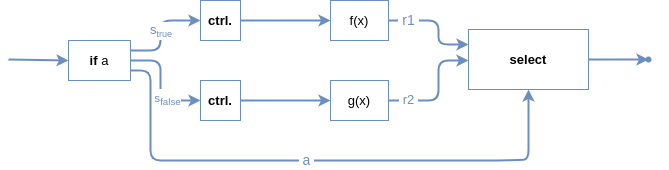
\includegraphics[height=3cm]{figures/branching_ohua.png}
     \label{subfig:branchingGraph}
    \end{subfigure}%
  }
  \cr
  \noalign{\hfill}
    \hbox{%
    \begin{subfigure}{.25\textwidth}
    \centering
     \begin{minted}[fontsize=\footnotesize]{rust}

     obj.do(x)

     \end{minted}
    \end{subfigure}    
    \begin{subfigure}{.72\textwidth}
    \centering
    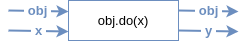
\includegraphics[height=1cm]{figures/method_ohua.png}
     \label{subfig:methodGraph}
    \end{subfigure}%
  }
  \cr
}
\caption{}
\label{fig:DFBranching}
\end{figure}

\subsection{The M\textsuperscript{3} Backend}

We currently run all nodes as separate processes on one tile. To leverage the full potential of M$^3$, we may change the backend implementation to actually allocate separate tiles for each process. As M$^3$ is designed to integrate different hardware components as tiles, this will be an interesting step towards supporting heterogeneous platforms. 

A limitation concerning the supported programming model is, that so far we did not implement the handling of environment variables, i.e. data initialized outside the algorithms and passed as arguments or just used in a shared scope. For the present example application, this was not an issue. We were compiling a \rust{main} function, which does not take input arguments. However we might want to also compile for libraries to M$^3$, where translated algorithms may need external input. How this can be implemented, depends on how the processes are created, i.e. on a single or multiple tiles and on whether the environment variable was defined inside the compile scope e.g. global constants or is actually passed in from processes calling the compiled code. In this context we will also need to evaluate whether its possible and necessary to generate the \code{xml} configuration files M$^3$ uses to declare interfaces and names of applications.  

Finally a problem that we will not be able to handle automatically is the translation of system service accesses, such are file system access, or the usage of device drivers. We saw for example, that we needed to adapt the implementation of \rust{phy_wait} based on M$^3$ implementations for network devices and process waiting. As described in Section~\ref{sec:FlexibleOSes} FlexOS and CubicleOS handle this problem by providing the programmer a) with a fixed set of supported libraries they can use and b) annotations for system calls, such as memory allocation the compiler can use to automatically replace system call appropriately for the target system. So likely for us adaptation to operating system features, other than the generation and direct communication of processes, will also rely on information from the programmer and the usage of suitable interfaces allready in the input code.

\subsection{Formalizing and Implementing Transformations}

\subsection{to be sorted somewhere}
\todo[inline]{States are not serializable \means we need to fuse all nodes using them OR we could derive a wrapper state that holds an Option<ActualState>. The \rust{process_call} function of this wrapper state would be the one of Option<ActualState> but augmented with a call to the initialization function }
\todo[inline]{ We do not have state threads for a) branching and b) recursion}
\todo[inline]{How to initialize variables integrated into the state?}

Remaining notes and question for 'automatization'
\begin{itemize}
    \item to support lambda lifting this way, a language needs to support sum type definition i.e.
    \code{type Functions = DoThis | DoThat | DoSomethingElse}
    Further difficulty: What traits do we need to derive? Obviously Clone and that needs to work because \means all arguments need to implement Clone. What else? Can we assume or derive automatically? 
    \item Bound variables, i.e. direct function arguments are just included in the function data types (as far as the language supports this, otherwise the Function type needs to represent any possible value of the arguments as individual type). In case of Rust, this is not a problem as sum types can be defined as \rust{enum}s which support additional data
    \item Free Variables, i.e. enclosed values from functions that where closures usually require lambda lifting. The term basically already describes the underlying principle, namely that free variables in a function are \emph{lifted} to the definition of the function as parameters i.e. bound by the lambda expression defining the function and the function itself is \emph{lifted} to a global scope. A simple example is shown in Figure~\ref{fig:lambdaLift}.
    \item process \means identify a) basic blocks b) data dependencies \means define function data types, arguments to constructors are data from other components \means define \rust{apply} function \means pattern matching on enums, code in match arms is code called directly before, if we were inside a state before, we need to retrieve and set the state to restore the behavior of the original 'closure'/subcall \means replace jumps and calls to other component with return \means overall return is union of original return and calls to other components
    \item If arguments follow the control flow they become part of the data type definition for the functions
    \item If arguments do not follow the control flow, i.e. if they belong to only one component, they are made part of the components state. This is particularly the case for the socket being processed in each round.
    \item particular issue occurring are lifetimes and ownership. Regardless whether we send values, or store them inside the state they must not reference each other. This is because we split a function, in this case \stack{.socket_egress} and thereby distribute execution that ran on one stack frame to multiple stack frames. As explained in the Background Section~\ref{subsec:Rust} this means that references, bound on the stack frame of one sub-function, can become invalid when the function exits and can not just be stored in the \stack{}s state for usage in the next sub-function. This becomes particularly obvious when we look at the loop over the sockets. 
    \item In the sequential program four references to the same object exist simultaneously i) the sockets, ii) the iterator on the sockets iii) the current socket and iv) the packet, which internally holds a reference to the sockets memory. 
\end{itemize}
